\documentclass[12pt]{beamer}
\usepackage{beamerthemeHannover, graphicx, clrscode, amsmath, amssymb, multicol}
\usepackage{textcomp} \usepackage{verbatim}
\usepackage{listings}
\setbeamercolor{sidebar}{use=structure,bg=purple}

\author[@dukeleto]{Jonathan "Duke" Leto\\\small{@dukeleto\\duke.leto.net\\duke@leto.net\\letolabs.com}}
\date{}
\title[PDXGit.clone()\hspace{2em}\insertframenumber/
\inserttotalframenumber]{Git Your City Together}
\setbeamertemplate{navigation symbols}{} %no nav symbols

% keynote-ish
\renewcommand\sfdefault{phv}
\renewcommand\familydefault{\sfdefault}
\usetheme{default}
\usepackage{color}
\useoutertheme{default}
%\usepackage{texnansi}
\usepackage{marvosym}
\definecolor{bottomcolour}{rgb}{0.32,0.3,0.38}
\definecolor{middlecolour}{rgb}{0.08,0.08,0.16}
\setbeamerfont{title}{size=\Huge}
\setbeamercolor{structure}{fg=gray}
\setbeamertemplate{frametitle}[default]%[center]
\setbeamercolor{normal text}{bg=black, fg=white}
\setbeamertemplate{background canvas}[vertical shading]
[bottom=bottomcolour, middle=middlecolour, top=black]
\setbeamertemplate{items}[circle]
\setbeamerfont{frametitle}{size=\huge}
\setbeamertemplate{navigation symbols}{} %no nav symbols

\begin{document}

\frame[t]{
    \begin{center}
            
\includegraphics[scale=0.15]{pdxgit-simantel-green}
    \end{center}
    \titlepage
}

\frame{
	\frametitle{ What You Will Learn }

	\begin{center}
	
		\includegraphics[scale=0.3]{spongebob_learning}

		\begin{itemize}
			\item How To Bootstrap
			\item How To Get Resources
			\item How To Be Sustainable
		\end{itemize}

	\end{center}
}


\frame{
    \frametitle{Origin Story}

	\begin{center}

	\includegraphics[scale=0.25]{first_meme}

	PDX Git was the *first* Git user group

    \begin{itemize}
        \item GSoC Mentor Summit Oct 2010
        \item Git Together Developer Conf Oct 2010
        \item GSoC Mentor Summit Oct 2011
        \item Git Together Developer Conf Oct 2011
        \item Feb 2012 1st PDXGit Meeting
    \end{itemize}

	\end{center}

}

\frame{
    \frametitle{Infrastructure}

    \begin{columns}
    \begin{column}{5cm}
        
\includegraphics[scale=0.5]{cat-tube}
    \end{column}
    \begin{column}{5cm}
        \begin{itemize}
            \item Github Pages
            \item Twitter Bootstrap
            \item Font Awesome
			\item Git!
        \end{itemize}
    \end{column}
    \end{columns}
}

\frame{
    \frametitle{Getting Free Stuff}
    \begin{columns}
        \begin{column}{5cm}
        
\includegraphics[scale=0.25]{free_tibet}
        \end{column}
        \begin{column}{5cm}
        \begin{itemize}
            \item Venue
            \item Food
            \item Schwag
            \item Publicity
        \end{itemize}
        \end{column}
    \end{columns}
}

\frame{
    \frametitle{Finding Sponsors}

        \begin{columns}
        \begin{column}{3cm}
			\includegraphics[scale=0.25]{404_meme}
        \end{column}

        \begin{column}{5cm}
			\begin{itemize}
				\item Who depends on Git?
				\item Who has a hiring frenzy?
				\item Who just got a funding round?
				\item Who is the "underdog"?
				\item Ask at other user groups
				\item Libraries/Community Center/Uni
				\item Local Mozillians
			\end{itemize}
		\end{column}
	\end{columns}
}

\frame{
    \frametitle{Self-Organizing Communities}
        \begin{columns}
        \begin{column}{5cm}
            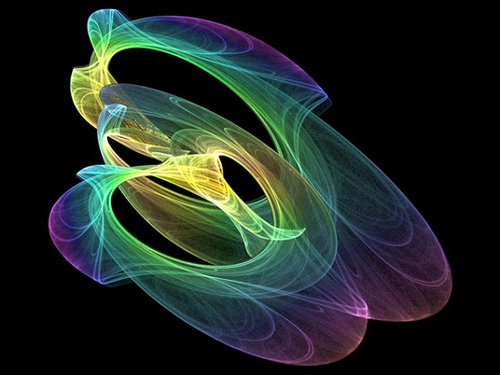
\includegraphics[scale=0.5]{lorenz}
        \end{column}
        \begin{column}{5cm}
            \begin{itemize}
                \item Embrace Chaos
                \item Foster Meritocracy
                \item Uphold Transparency
            \end{itemize}
        \end{column}
       \end{columns}
}

\frame{
    \frametitle{Community Guidelines}
        \begin{columns}
        \begin{column}{5cm}
            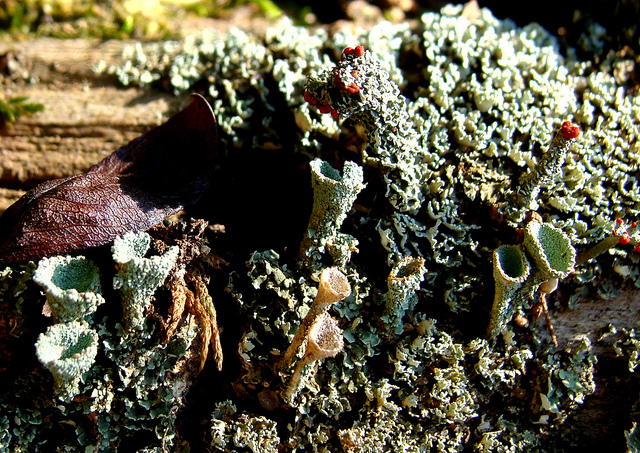
\includegraphics[scale=0.25]{lichen}
        \end{column}
        \begin{column}{5cm}
            \begin{itemize}
                \item Define  Publicly
                \item Modify  Publicly
                \item Enforce Publicly
            \end{itemize}
        \end{column}
       \end{columns}
}

\frame{
    \frametitle{Stay Sustainable}
    \begin{itemize}
        \item Rotating leadership
        \item Focused Projects
		\item Mix Things Up
    \end{itemize}
}

\frame{
    \frametitle{Meeting Formats}

    \begin{itemize}
        \item One Long Talk
        \item Lots of Small Talks
        \item Two or three 15/20 minute slots
        \item Co-hacking
		\item Social
    \end{itemize}
}

\frame{
    \frametitle{Checklist 1/2}

	Up and going in 10 minutes

    \begin{itemize}
        \item Create a Github Org for your Clone
        \item Fork github.com/pdxgit/pdxgit.github.com
        \item Rename your repo ORG/NAME.github.io
		\item Update links (s/pdxgit/yourgroup/g)
    \end{itemize}
}

\frame{
    \frametitle{Checklist 2/2}

	Optimizations

    \begin{itemize}
        \item Register a domain
        \item Change CNAME file to be your domain
        \item Configure DNS $ \to $ Github Pages
        \item Create a Google/FB/LinkedIn etc Group
    \end{itemize}
}

\frame{
	\frametitle{/dev/random Tips}

    \begin{itemize}
		\item Don't Do Everything
        \item Align With Conferences
	    \item Have Fun
    \end{itemize}

	\includegraphics[scale=0.63]{random_meme}
}

\frame{
    \frametitle{The Usual Suspects}

	\includegraphics[scale=0.1]{usual_suspects}

	Without these people @pdxgit would not be possible

    \begin{itemize}
		\item Ben Cullen-Kerney - @beancuke (website)
		\item Bart Massey (logo and advice)
		\item Ben Hengst
		\item Christopher Swenson

    \end{itemize}
}

\frame{
	\frametitle{Dedication}

	\begin{center}
	\includegraphics[scale=0.75]{igal_and_caterpillar} \\
	Igal Koshevoy - @igalko

	\end{center}
}

\frame{
    \frametitle{git merge -s=social}
    \begin{columns}
		\begin{column}{5cm}
			\includegraphics[scale=0.25]{letolabs}
		\end{column}
		\begin{column}{5cm}
			\begin{itemize}
			\item @dukeleto
			\item duke.leto.net
			\item duke@leto.net
			\item linkedin.leto.net
			\item IRC: dukeleto
			\item Github: @leto
			\item 209.691.DUKE
			\end{itemize}
		\end{column}
    \end{columns}
}

\frame{
    \frametitle{Mahalo!}
	\begin{center}
		
\includegraphics[scale=1.5]{pdxgit}
	\end{center}
}
\end{document}
